\documentclass[12pt]{article}
%Gummi|065|=)
\usepackage{amsmath, amsfonts, amssymb}
\usepackage[margin=0.5in]{geometry}
\usepackage{xcolor}
\usepackage{graphicx}
%\usepackage{graphicx}
\newcommand{\off}[1]{}
\DeclareMathSizes{20}{30}{20}{18}
\newcommand{\myhrule}{}

\newcommand{\two }{\sqrt[3]{2}}
\newcommand{\four}{\sqrt[3]{4}}

\newcommand{\dash}{
\begin{tikzpicture}[scale=1]
\draw (0,0)--(19,0);
\end{tikzpicture}
}

\newcommand{\sq}[3]{
\node at (#1+0.5,#2+0.5) {#3};
\draw (#1+0,#2+0)--(#1+1,#2+0)--(#1+1,#2+1)--(#1+0,#2+1)--cycle;
}

\usepackage{tikz}

\title{\textbf{Proposal: Factorial}}
\author{John D Mangual}
\date{}
\begin{document}

\fontfamily{qag}\selectfont \fontsize{20}{25}\selectfont

\maketitle

\noindent Some clever person turned the theory domino tilings into a fundamental object of mathematics and of nature.  For a long time there were really two shapes being studied.  \\ \\
The rectangle (here an $8 \times 8$ square): \\
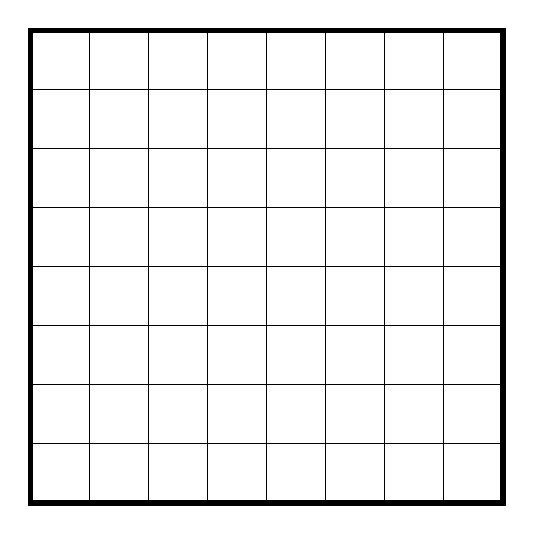
\begin{tikzpicture}[scale=0.75]

\foreach \a in {0,...,8}{
	\draw (\a,0)--(\a,8);
	\draw (0,\a)--(8,\a);
}

\draw[line width = 2] (0,0)--(8,0)--(8,8)--(0,8)--cycle;

\end{tikzpicture} \\ 
And I wonder why this particular shape is so essential: \\
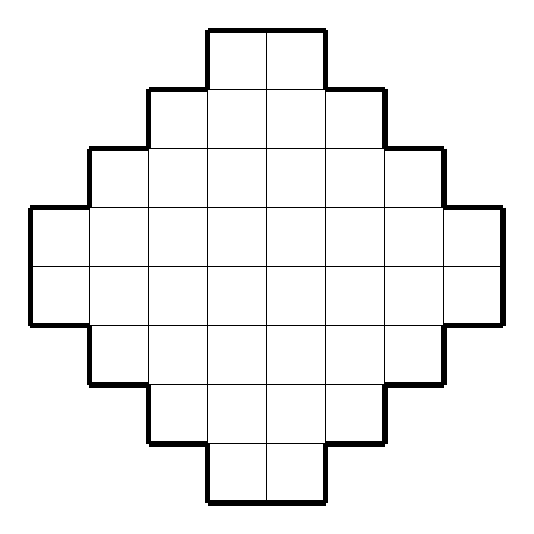
\begin{tikzpicture}[scale=0.75]



\foreach \a in {0,...,3}{

	\draw[line width=2] (\a  ,4-\a)--(\a+1, 4-\a  );
	\draw[line width=2] (\a+1,4-\a)--(\a+1, 4-\a-1);
	
	\draw (   \a, 4-\a)--(   \a, \a-4);
	\draw (-1*\a, 4-\a)--(-1*\a, \a-4);
	
	\draw ( 4-\a,    \a)--(\a-4,    \a);
	\draw ( 4-\a, -1*\a)--(\a-4, -1*\a);

	\def \b {-1}
	\def \c { 1}
		
	\draw[line width=2] (\b*\a  ,\c*4-\c*\a)--(\b*\a+\b*1, \c*4-\c*\a  );
	\draw[line width=2] (\b*\a+\b*1,\c*4-\c*\a)--(\b*\a+\b*1, \c*4-\c*\a-\c*1);
	
	\def \b { 1}
	\def \c {-1}
		
	\draw[line width=2] (\b*\a  ,\c*4-\c*\a)--(\b*\a+\b*1, \c*4-\c*\a  );
	\draw[line width=2] (\b*\a+\b*1,\c*4-\c*\a)--(\b*\a+\b*1, \c*4-\c*\a-\c*1);
	
	\def \b {-1}
	\def \c {-1}
		
	\draw[line width=2] (\b*\a  ,\c*4-\c*\a)--(\b*\a+\b*1, \c*4-\c*\a  );
	\draw[line width=2] (\b*\a+\b*1,\c*4-\c*\a)--(\b*\a+\b*1, \c*4-\c*\a-\c*1);

}

\end{tikzpicture}

\newpage

\noindent Pathetic Tutorial:

\fontfamily{qag}\selectfont \fontsize{12}{10}\selectfont

\begin{verbatim}
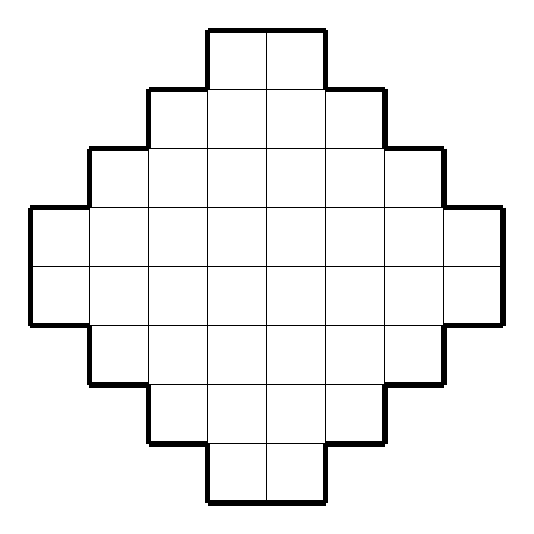
\begin{tikzpicture}[scale=0.75]

\foreach \a in {0,...,3}{

	\draw[line width=2] (\a  ,4-\a)--(\a+1, 4-\a  );
	\draw[line width=2] (\a+1,4-\a)--(\a+1, 4-\a-1);
	
	\draw (   \a, 4-\a)--(   \a, \a-4);
	\draw (-1*\a, 4-\a)--(-1*\a, \a-4);
	
	\draw ( 4-\a,    \a)--(\a-4,    \a);
	\draw ( 4-\a, -1*\a)--(\a-4, -1*\a);

	\def \b {-1}
	\def \c { 1}
		
	\draw[line width=2] (\b*\a     ,\c*4-\c*\a)--(\b*\a+\b*1, \c*4-\c*\a     );
	\draw[line width=2] (\b*\a+\b*1,\c*4-\c*\a)--(\b*\a+\b*1, \c*4-\c*\a-\c*1);
	
	\def \b { 1}
	\def \c {-1}
		
	\draw[line width=2] (\b*\a     ,\c*4-\c*\a)--(\b*\a+\b*1, \c*4-\c*\a     );
	\draw[line width=2] (\b*\a+\b*1,\c*4-\c*\a)--(\b*\a+\b*1, \c*4-\c*\a-\c*1);
	
	\def \b {-1}
	\def \c {-1}
		
	\draw[line width=2] (\b*\a     ,\c*4-\c*\a)--(\b*\a+\b*1, \c*4-\c*\a     );
	\draw[line width=2] (\b*\a+\b*1,\c*4-\c*\a)--(\b*\a+\b*1, \c*4-\c*\a-\c*1);

}

\end{tikzpicture}

\end{verbatim}


\noindent In French the word for tiling is \textit{pavage} -- so literally we are \textbf{paving} the shapes with dominoes. 




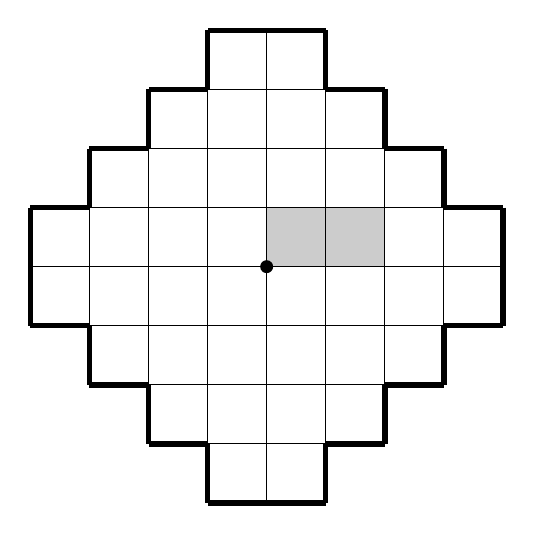
\begin{tikzpicture}[scale=0.75]

\def \b {0}
\def \c {0}


\draw[fill=black!20!white] (\b,\c)--(\b+2,\c)--(\b+2,\c+1)--(\b,\c+1)--cycle;
\draw[fill=black] (\b,\c) circle (0.1);

\foreach \a in {0,...,3}{

	\draw[line width=2] (\a  ,4-\a)--(\a+1, 4-\a  );
	\draw[line width=2] (\a+1,4-\a)--(\a+1, 4-\a-1);
	
	\draw (   \a, 4-\a)--(   \a, \a-4);
	\draw (-1*\a, 4-\a)--(-1*\a, \a-4);
	
	\draw ( 4-\a,    \a)--(\a-4,    \a);
	\draw ( 4-\a, -1*\a)--(\a-4, -1*\a);

	\def \b {-1}
	\def \c { 1}
		
	\draw[line width=2] (\b*\a  ,\c*4-\c*\a)--(\b*\a+\b*1, \c*4-\c*\a  );
	\draw[line width=2] (\b*\a+\b*1,\c*4-\c*\a)--(\b*\a+\b*1, \c*4-\c*\a-\c*1);
	
	\def \b { 1}
	\def \c {-1}
		
	\draw[line width=2] (\b*\a  ,\c*4-\c*\a)--(\b*\a+\b*1, \c*4-\c*\a  );
	\draw[line width=2] (\b*\a+\b*1,\c*4-\c*\a)--(\b*\a+\b*1, \c*4-\c*\a-\c*1);
	
	\def \b {-1}
	\def \c {-1}
		
	\draw[line width=2] (\b*\a  ,\c*4-\c*\a)--(\b*\a+\b*1, \c*4-\c*\a  );
	\draw[line width=2] (\b*\a+\b*1,\c*4-\c*\a)--(\b*\a+\b*1, \c*4-\c*\a-\c*1);

}

\end{tikzpicture}

\newpage

\noindent Let's put two reasonable tilings on the board.  One strategy for this shape is to start from the corners and work indwards.  And in this case we get lucky: it always works. \\

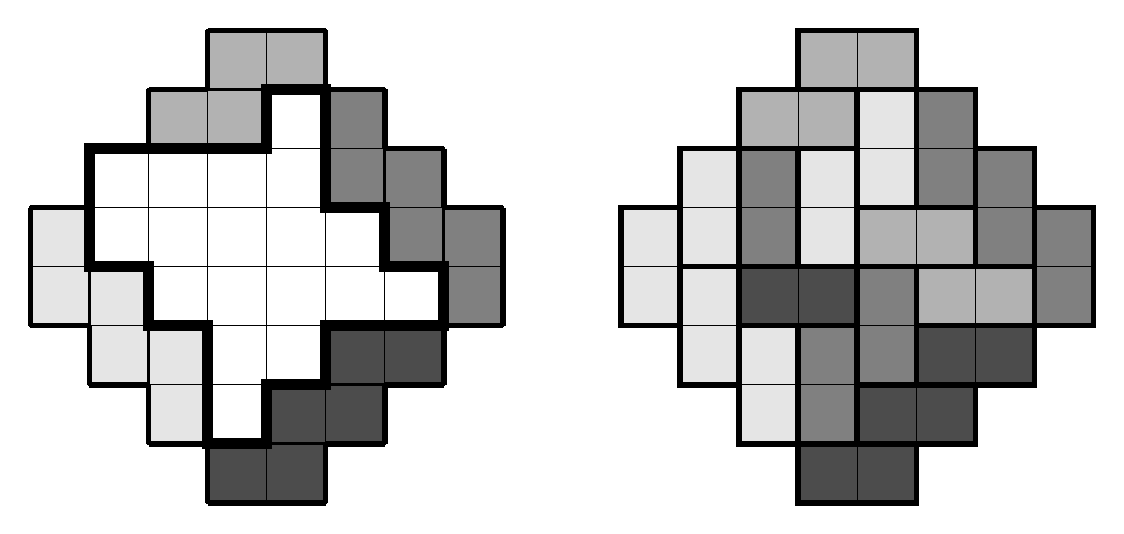
\begin{tikzpicture}[scale=0.75]


%\def \b {0}
%\def \c {0}
%\draw[fill=black!30!white, line width=2] (\b,\c)--(\b+2,\c)--(\b+2,\c+1)--(\b,\c+1)--cycle;

\def \b {-1}
\def \c {3}
\draw[fill=black!30!white, line width=1] (\b,\c)--(\b+2,\c)--(\b+2,\c+1)--(\b,\c+1)--cycle;

\def \b {-2}
\def \c {2}
\draw[fill=black!30!white, line width=1] (\b,\c)--(\b+2,\c)--(\b+2,\c+1)--(\b,\c+1)--cycle;

\def \b {-1}
\def \c {-4}
\draw[fill=black!70!white, line width=1] (\b,\c)--(\b+2,\c)--(\b+2,\c+1)--(\b,\c+1)--cycle;

\def \b {0}
\def \c {-3}
\draw[fill=black!70!white, line width=1] (\b,\c)--(\b+2,\c)--(\b+2,\c+1)--(\b,\c+1)--cycle;

\def \b {1}
\def \c {-2}
\draw[fill=black!70!white, line width=1] (\b,\c)--(\b+2,\c)--(\b+2,\c+1)--(\b,\c+1)--cycle;

\def \b {-4}
\def \c {-1}
\draw[fill=black!10!white, line width=1] (\b,\c)--(\b+1,\c)--(\b+1,\c+2)--(\b,\c+2)--cycle;

\def \b {-3}
\def \c {-2}
\draw[fill=black!10!white, line width=1] (\b,\c)--(\b+1,\c)--(\b+1,\c+2)--(\b,\c+2)--cycle;

\def \b {-2}
\def \c {-3}
\draw[fill=black!10!white, line width=1] (\b,\c)--(\b+1,\c)--(\b+1,\c+2)--(\b,\c+2)--cycle;

%\def \b {-3}
%\def \c {0}
%\draw[fill=black!10!white, line width=2] (\b,\c)--(\b+1,\c)--(\b+1,\c+2)--(\b,\c+2)--cycle;

\def \b {1}
\def \c {1}
\draw[fill=black!50!white, line width=1] (\b,\c)--(\b+1,\c)--(\b+1,\c+2)--(\b,\c+2)--cycle;

\def \b {2}
\def \c {0}
\draw[fill=black!50!white, line width=1] (\b,\c)--(\b+1,\c)--(\b+1,\c+2)--(\b,\c+2)--cycle;

\def \b {3}
\def \c {-1}
\draw[fill=black!50!white, line width=1] (\b,\c)--(\b+1,\c)--(\b+1,\c+2)--(\b,\c+2)--cycle;



\foreach \a in {0,...,3}{

	\draw[line width=2] (\a  ,4-\a)--(\a+1, 4-\a  );
	\draw[line width=2] (\a+1,4-\a)--(\a+1, 4-\a-1);
	
	\draw (   \a, 4-\a)--(   \a, \a-4);
	\draw (-1*\a, 4-\a)--(-1*\a, \a-4);
	
	\draw ( 4-\a,    \a)--(\a-4,    \a);
	\draw ( 4-\a, -1*\a)--(\a-4, -1*\a);

	\def \b {-1}
	\def \c { 1}
		
	\draw[line width=2] (\b*\a  ,\c*4-\c*\a)--(\b*\a+\b*1, \c*4-\c*\a  );
	\draw[line width=2] (\b*\a+\b*1,\c*4-\c*\a)--(\b*\a+\b*1, \c*4-\c*\a-\c*1);
	
	\def \b { 1}
	\def \c {-1}
		
	\draw[line width=2] (\b*\a  ,\c*4-\c*\a)--(\b*\a+\b*1, \c*4-\c*\a  );
	\draw[line width=2] (\b*\a+\b*1,\c*4-\c*\a)--(\b*\a+\b*1, \c*4-\c*\a-\c*1);
	
	\def \b {-1}
	\def \c {-1}
		
	\draw[line width=2] (\b*\a  ,\c*4-\c*\a)--(\b*\a+\b*1, \c*4-\c*\a  );
	\draw[line width=2] (\b*\a+\b*1,\c*4-\c*\a)--(\b*\a+\b*1, \c*4-\c*\a-\c*1);

}

\draw[line width=4] (0,-2)--(1,-2)--(1,-1)--(3,-1)--(3,0)--(2,0)--(2,1)--(1,1)--(1,3)--(0,3)--(0,2)--(-3,2)--(-3,0)--(-2,0)--(-2,-1)--(-1,-1)--(-1,-3)--(0,-3)--cycle;

\begin{scope}[xshift=10cm]

%\def \b {0}
%\def \c {0}
%\draw[fill=black!30!white, line width=2] (\b,\c)--(\b+2,\c)--(\b+2,\c+1)--(\b,\c+1)--cycle;

\def \b {-1}
\def \c {3}
\draw[fill=black!30!white, line width=2] (\b,\c)--(\b+2,\c)--(\b+2,\c+1)--(\b,\c+1)--cycle;

\def \b {-2}
\def \c {2}
\draw[fill=black!30!white, line width=2] (\b,\c)--(\b+2,\c)--(\b+2,\c+1)--(\b,\c+1)--cycle;

\def \b {1}
\def \c {-1}
\draw[fill=black!30!white, line width=2] (\b,\c)--(\b+2,\c)--(\b+2,\c+1)--(\b,\c+1)--cycle;

\def \b {0}
\def \c {0}
\draw[fill=black!30!white, line width=2] (\b,\c)--(\b+2,\c)--(\b+2,\c+1)--(\b,\c+1)--cycle;

\def \b {-1}
\def \c {-4}
\draw[fill=black!70!white, line width=2] (\b,\c)--(\b+2,\c)--(\b+2,\c+1)--(\b,\c+1)--cycle;

\def \b {0}
\def \c {-3}
\draw[fill=black!70!white, line width=2] (\b,\c)--(\b+2,\c)--(\b+2,\c+1)--(\b,\c+1)--cycle;

\def \b {1}
\def \c {-2}
\draw[fill=black!70!white, line width=2] (\b,\c)--(\b+2,\c)--(\b+2,\c+1)--(\b,\c+1)--cycle;

\def \b {-2}
\def \c {-1}
\draw[fill=black!70!white, line width=2] (\b,\c)--(\b+2,\c)--(\b+2,\c+1)--(\b,\c+1)--cycle;

\def \b {-4}
\def \c {-1}
\draw[fill=black!10!white, line width=2] (\b,\c)--(\b+1,\c)--(\b+1,\c+2)--(\b,\c+2)--cycle;

\def \b {-3}
\def \c {-2}
\draw[fill=black!10!white, line width=2] (\b,\c)--(\b+1,\c)--(\b+1,\c+2)--(\b,\c+2)--cycle;

\def \b {-2}
\def \c {-3}
\draw[fill=black!10!white, line width=2] (\b,\c)--(\b+1,\c)--(\b+1,\c+2)--(\b,\c+2)--cycle;

\def \b {0}
\def \c {1}
\draw[fill=black!10!white, line width=2] (\b,\c)--(\b+1,\c)--(\b+1,\c+2)--(\b,\c+2)--cycle;

\def \b {-3}
\def \c {0}
\draw[fill=black!10!white, line width=2] (\b,\c)--(\b+1,\c)--(\b+1,\c+2)--(\b,\c+2)--cycle;

\def \b {-1}
\def \c {0}
\draw[fill=black!10!white, line width=2] (\b,\c)--(\b+1,\c)--(\b+1,\c+2)--(\b,\c+2)--cycle;

\def \b {1}
\def \c {1}
\draw[fill=black!50!white, line width=2] (\b,\c)--(\b+1,\c)--(\b+1,\c+2)--(\b,\c+2)--cycle;

\def \b {2}
\def \c {0}
\draw[fill=black!50!white, line width=2] (\b,\c)--(\b+1,\c)--(\b+1,\c+2)--(\b,\c+2)--cycle;

\def \b {3}
\def \c {-1}
\draw[fill=black!50!white, line width=2] (\b,\c)--(\b+1,\c)--(\b+1,\c+2)--(\b,\c+2)--cycle;

\def \b {-2}
\def \c {0}
\draw[fill=black!50!white, line width=2] (\b,\c)--(\b+1,\c)--(\b+1,\c+2)--(\b,\c+2)--cycle;

\def \b {-1}
\def \c {-3}
\draw[fill=black!50!white, line width=2] (\b,\c)--(\b+1,\c)--(\b+1,\c+2)--(\b,\c+2)--cycle;

\def \b {0}
\def \c {-2}
\draw[fill=black!50!white, line width=2] (\b,\c)--(\b+1,\c)--(\b+1,\c+2)--(\b,\c+2)--cycle;

\foreach \a in {0,...,3}{

	\draw[line width=2] (\a  ,4-\a)--(\a+1, 4-\a  );
	\draw[line width=2] (\a+1,4-\a)--(\a+1, 4-\a-1);
	
	\draw (   \a, 4-\a)--(   \a, \a-4);
	\draw (-1*\a, 4-\a)--(-1*\a, \a-4);
	
	\draw ( 4-\a,    \a)--(\a-4,    \a);
	\draw ( 4-\a, -1*\a)--(\a-4, -1*\a);

	\def \b {-1}
	\def \c { 1}
		
	\draw[line width=2] (\b*\a  ,\c*4-\c*\a)--(\b*\a+\b*1, \c*4-\c*\a  );
	\draw[line width=2] (\b*\a+\b*1,\c*4-\c*\a)--(\b*\a+\b*1, \c*4-\c*\a-\c*1);
	
	\def \b { 1}
	\def \c {-1}
		
	\draw[line width=2] (\b*\a  ,\c*4-\c*\a)--(\b*\a+\b*1, \c*4-\c*\a  );
	\draw[line width=2] (\b*\a+\b*1,\c*4-\c*\a)--(\b*\a+\b*1, \c*4-\c*\a-\c*1);
	
	\def \b {-1}
	\def \c {-1}
		
	\draw[line width=2] (\b*\a  ,\c*4-\c*\a)--(\b*\a+\b*1, \c*4-\c*\a  );
	\draw[line width=2] (\b*\a+\b*1,\c*4-\c*\a)--(\b*\a+\b*1, \c*4-\c*\a-\c*1);

}

\end{scope}

\end{tikzpicture} \\ 

\noindent And for rectangle the case is even clearer.  There are no intermediate stages.  I mean, if you put enough tiles down there can be come question as to whether you put yourself in a corner yet.   \\ \\

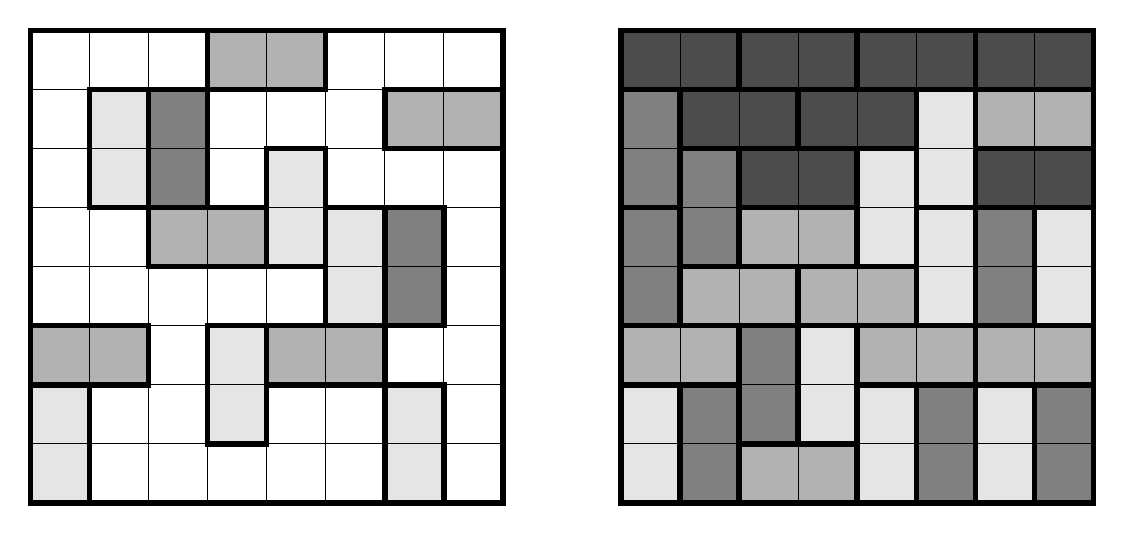
\begin{tikzpicture}[scale=0.75]

\def \b {0}
\def \c {0}
\draw[fill=black!10!white, line width=2] (\b,\c)--(\b+1,\c)--(\b+1,\c+2)--(\b,\c+2)--cycle;

\def \b {3}
\def \c {1}
\draw[fill=black!10!white, line width=2] (\b,\c)--(\b+1,\c)--(\b+1,\c+2)--(\b,\c+2)--cycle;

\def \b {4}
\def \c {4}
\draw[fill=black!10!white, line width=2] (\b,\c)--(\b+1,\c)--(\b+1,\c+2)--(\b,\c+2)--cycle;

\def \b {5}
\def \c {3}
\draw[fill=black!10!white, line width=2] (\b,\c)--(\b+1,\c)--(\b+1,\c+2)--(\b,\c+2)--cycle;

\def \b {6}
\def \c {0}
\draw[fill=black!10!white, line width=2] (\b,\c)--(\b+1,\c)--(\b+1,\c+2)--(\b,\c+2)--cycle;

\def \b {1}
\def \c {5}
\draw[fill=black!10!white, line width=2] (\b,\c)--(\b+1,\c)--(\b+1,\c+2)--(\b,\c+2)--cycle;

\def \b {0}
\def \c {2}
\draw[fill=black!30!white, line width=2] (\b,\c)--(\b+2,\c)--(\b+2,\c+1)--(\b,\c+1)--cycle;

\def \b {2}
\def \c {4}
\draw[fill=black!30!white, line width=2] (\b,\c)--(\b+2,\c)--(\b+2,\c+1)--(\b,\c+1)--cycle;

\def \b {3}
\def \c {7}
\draw[fill=black!30!white, line width=2] (\b,\c)--(\b+2,\c)--(\b+2,\c+1)--(\b,\c+1)--cycle;

\def \b {6}
\def \c {6}
\draw[fill=black!30!white, line width=2] (\b,\c)--(\b+2,\c)--(\b+2,\c+1)--(\b,\c+1)--cycle;

\def \b {4}
\def \c {2}
\draw[fill=black!30!white, line width=2] (\b,\c)--(\b+2,\c)--(\b+2,\c+1)--(\b,\c+1)--cycle;

\def \b {6}
\def \c {3}
\draw[fill=black!50!white, line width=2] (\b,\c)--(\b+1,\c)--(\b+1,\c+2)--(\b,\c+2)--cycle;

\def \b {2}
\def \c {5}
\draw[fill=black!50!white, line width=2] (\b,\c)--(\b+1,\c)--(\b+1,\c+2)--(\b,\c+2)--cycle;

\foreach \a in {0,...,8}{
	\draw (\a,0)--(\a,8);
	\draw (0,\a)--(8,\a);
}

\draw[line width = 2] (0,0)--(8,0)--(8,8)--(0,8)--cycle;



\begin{scope}[xshift=10cm]

\def \b {0}
\def \c {0}
\draw[fill=black!10!white, line width=2] (\b,\c)--(\b+1,\c)--(\b+1,\c+2)--(\b,\c+2)--cycle;

\def \b {3}
\def \c {1}
\draw[fill=black!10!white, line width=2] (\b,\c)--(\b+1,\c)--(\b+1,\c+2)--(\b,\c+2)--cycle;

\def \b {4}
\def \c {4}
\draw[fill=black!10!white, line width=2] (\b,\c)--(\b+1,\c)--(\b+1,\c+2)--(\b,\c+2)--cycle;

\def \b {5}
\def \c {3}
\draw[fill=black!10!white, line width=2] (\b,\c)--(\b+1,\c)--(\b+1,\c+2)--(\b,\c+2)--cycle;

\def \b {6}
\def \c {0}
\draw[fill=black!10!white, line width=2] (\b,\c)--(\b+1,\c)--(\b+1,\c+2)--(\b,\c+2)--cycle;

\def \b {1}
\def \c {5}
%\draw[fill=black!10!white, line width=2] (\b,\c)--(\b+1,\c)--(\b+1,\c+2)--(\b,\c+2)--cycle;

\def \b {0}
\def \c {2}
\draw[fill=black!30!white, line width=2] (\b,\c)--(\b+2,\c)--(\b+2,\c+1)--(\b,\c+1)--cycle;

\def \b {2}
\def \c {4}
\draw[fill=black!30!white, line width=2] (\b,\c)--(\b+2,\c)--(\b+2,\c+1)--(\b,\c+1)--cycle;

\def \b {2}
\def \c {7}
\draw[fill=black!70!white, line width=2] (\b,\c)--(\b+2,\c)--(\b+2,\c+1)--(\b,\c+1)--cycle;


\def \b {4}
\def \c {7}
\draw[fill=black!70!white, line width=2] (\b,\c)--(\b+2,\c)--(\b+2,\c+1)--(\b,\c+1)--cycle;

\def \b {3}
\def \c {6}
\draw[fill=black!70!white, line width=2] (\b,\c)--(\b+2,\c)--(\b+2,\c+1)--(\b,\c+1)--cycle;

\def \b {2}
\def \c {5}
\draw[fill=black!70!white, line width=2] (\b,\c)--(\b+2,\c)--(\b+2,\c+1)--(\b,\c+1)--cycle;

\def \b {1}
\def \c {6}
\draw[fill=black!70!white, line width=2] (\b,\c)--(\b+2,\c)--(\b+2,\c+1)--(\b,\c+1)--cycle;

\def \b {0}
\def \c {7}
\draw[fill=black!70!white, line width=2] (\b,\c)--(\b+2,\c)--(\b+2,\c+1)--(\b,\c+1)--cycle;


\def \b {6}
\def \c {6}
\draw[fill=black!30!white, line width=2] (\b,\c)--(\b+2,\c)--(\b+2,\c+1)--(\b,\c+1)--cycle;

\def \b {4}
\def \c {2}
\draw[fill=black!30!white, line width=2] (\b,\c)--(\b+2,\c)--(\b+2,\c+1)--(\b,\c+1)--cycle;

\def \b {6}
\def \c {3}
\draw[fill=black!50!white, line width=2] (\b,\c)--(\b+1,\c)--(\b+1,\c+2)--(\b,\c+2)--cycle;

\def \b {2}
\def \c {5}
%\draw[fill=black!50!white, line width=2] (\b,\c)--(\b+1,\c)--(\b+1,\c+2)--(\b,\c+2)--cycle;

\def \b {7}
\def \c {0}
\draw[fill=black!50!white, line width=2] (\b,\c)--(\b+1,\c)--(\b+1,\c+2)--(\b,\c+2)--cycle;

\def \b {6}
\def \c {2}
\draw[fill=black!30!white, line width=2] (\b,\c)--(\b+2,\c)--(\b+2,\c+1)--(\b,\c+1)--cycle;

\def \b {7}
\def \c {3}
\draw[fill=black!10!white, line width=2] (\b,\c)--(\b+1,\c)--(\b+1,\c+2)--(\b,\c+2)--cycle;

\def \b {6}
\def \c {5}
\draw[fill=black!70!white, line width=2] (\b,\c)--(\b+2,\c)--(\b+2,\c+1)--(\b,\c+1)--cycle;

\def \b {6}
\def \c {7}
\draw[fill=black!70!white, line width=2] (\b,\c)--(\b+2,\c)--(\b+2,\c+1)--(\b,\c+1)--cycle;

\def \b {5}
\def \c {5}
\draw[fill=black!10!white, line width=2] (\b,\c)--(\b+1,\c)--(\b+1,\c+2)--(\b,\c+2)--cycle;

\def \b {5}
\def \c {0}
\draw[fill=black!50!white, line width=2] (\b,\c)--(\b+1,\c)--(\b+1,\c+2)--(\b,\c+2)--cycle;

\def \b {4}
\def \c {0}
\draw[fill=black!10!white, line width=2] (\b,\c)--(\b+1,\c)--(\b+1,\c+2)--(\b,\c+2)--cycle;

\def \b {3}
\def \c {3}
\draw[fill=black!30!white, line width=2] (\b,\c)--(\b+2,\c)--(\b+2,\c+1)--(\b,\c+1)--cycle;

\def \b {2}
\def \c {0}
\draw[fill=black!30!white, line width=2] (\b,\c)--(\b+2,\c)--(\b+2,\c+1)--(\b,\c+1)--cycle;

\def \b {1}
\def \c {0}
\draw[fill=black!50!white, line width=2] (\b,\c)--(\b+1,\c)--(\b+1,\c+2)--(\b,\c+2)--cycle;

\def \b {2}
\def \c {1}
\draw[fill=black!50!white, line width=2] (\b,\c)--(\b+1,\c)--(\b+1,\c+2)--(\b,\c+2)--cycle;

\def \b {1}
\def \c {3}
\draw[fill=black!30!white, line width=2] (\b,\c)--(\b+2,\c)--(\b+2,\c+1)--(\b,\c+1)--cycle;

\def \b {0}
\def \c {3}
\draw[fill=black!50!white, line width=2] (\b,\c)--(\b+1,\c)--(\b+1,\c+2)--(\b,\c+2)--cycle;

\def \b {0}
\def \c {5}
\draw[fill=black!50!white, line width=2] (\b,\c)--(\b+1,\c)--(\b+1,\c+2)--(\b,\c+2)--cycle;

\def \b {1}
\def \c {4}
\draw[fill=black!50!white, line width=2] (\b,\c)--(\b+1,\c)--(\b+1,\c+2)--(\b,\c+2)--cycle;

\foreach \a in {0,...,8}{
	\draw (\a,0)--(\a,8);
	\draw (0,\a)--(8,\a);
}

\draw[line width = 2] (0,0)--(8,0)--(8,8)--(0,8)--cycle;

\end{scope}


\end{tikzpicture} \\ \\
There is also the lovely John Conway game of ``Domineering" which is not related but you also place dominoes on a checkerboard. See \textbf{Winning Ways for Your Mathematical Plays} (Vol I). \\ \\
\textbf{Exercise} Fill the rest of the tiling. \\ \\
\textbf{Answer} There is no solution, but if you move the tiles slightly (actually quite a bit here...) you can get a problem with an answer.  \\ \\
The number of tilings on the top looks atypical -- just purely on a hunch.  Where did that hunch come from? Is it right? \\ \\
As with all hunches, it can be proven with hundreds of pages of equations this tiling is not likely to appear in a rectangles.  We'll settle for somewhat simpler patterns. 

\newpage

\noindent 

\newpage 

\noindent Next I hav to address some redundancy.  Every couple of years, it seems there were more and more people who came up with a similar theory and did not talk to each other.



\begin{itemize}
\item \textbf{domino tilings} 
\item dimer model 
\item perfect matchings
\item \textbf{six-vertex  model}
\item Alternating Sign Matrix (\textbf{ASM})
\item XXZ spin chain
\item Ising model
\end{itemize}

\noindent Domino tilings and six-vertex are closely related.  You can see the family resemblance.  

\includegraphics[width=5in]{AD-05.png} \\

\noindent For every 6-vertex configuration there is a domino tiling, up to various factors of $\times 2$.  

\includegraphics[width=5in]{AD-06.png}\\
The Aztec Diamond is a natural shape because it \textbf{is} the square lattice.

\newpage

\fontfamily{qag}\selectfont \fontsize{20}{25}\selectfont  

\noindent \textbf{Problem Session} Let us compute some square-ice and domino tiling partition functions! 

\newpage

\fontfamily{qag}\selectfont \fontsize{12}{10}\selectfont

\begin{thebibliography}{}

\item Paul Zinn-Justin \textbf{Six-Vertex Model with Domain Wall Boundary Conditions and One-Matrix Model} \texttt{arXiv:math-ph/0005008}

\item Noam Elkies, Greg Kuperberg, Michael Larsen, James Propp \\ \textbf{Alternating-Sign Matrices and Domino Tilings (Part I) }  \\ Journal of Algebraic Combinatorics (1992) 1: 111.  \texttt{doi:10.1023/A:1022420103267}

\item Sunil Chhita, Kurt Johansson \textbf{Domino statistics of the two-periodic Aztec diamond} \texttt{arXiv:1410.2385
}

\end{thebibliography} 

\newpage

\noindent The most amazing typo ever: \\

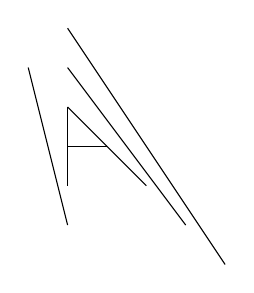
\begin{tikzpicture} [scale=0.5]

\foreach \a in {0,...,5}{
    \draw (\a,5-\a)--(1, \a + 1);
}

\end{tikzpicture}

\begin{verbatim}
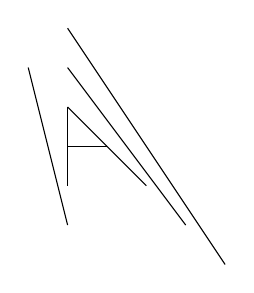
\begin{tikzpicture} [scale=0.5]

\foreach \a in {0,...,5}{

    \draw (\a, 5-\a)--(1, \a + 1);

}

\end{tikzpicture}
\end{verbatim}

\end{document}